\chapter{Design} \label{chapter:design}
During the design stage, we set out research questions and detail the steps of the machine learning pipeline for diagnosing fault types in the MaFaulDa dataset. The explanatory analysis of MaFaulDa hints at the underlying dependencies with feature sets that can degrade the machine learning model of choice. We adapt the methodology for measurements from standards and apply it to data logger requirements and data acquisition from industrial equipment.

\section{Research questions}
The thesis aims to provide answers to four research questions. The focus is primarily on making data flow more efficient in an industrial sensor network that monitors rotating machines. The \textbf{research questions} are:
\begin{enumerate}[label=RQ\arabic*., font=\bfseries]
    \itemsep0pt
	\item Which temporal and spectral features can be extracted from vibration signals to provide the most accurate record of machinery faults?
	\item What is the reduction in transmission goodput when chosen signal features are used?
	\item What accuracy of prediction models can be achieved with various feature subsets?
	\item How can machinery faults be continuously identified and predicted based upon collected events?
\end{enumerate}

\noindent In accomplishing the objectives of our research we propose several \textbf{goals}:
\begin{todolist}
    \itemsep0pt
    \item Statistically and visually describe vibration signals from the Machinery fault database (MauFaulDa).
    \item Establish a list of conditions that should be later investigated in the experimental setting.
    \item Prepare dataset to be used in conjunction with machine learning models, namely by identifying labels and balancing classes.
    \item Find the best subsets of features in the time and frequnecy domain with previously analyzed feature extraction and selection methods.
    \item Evaluate the performance of models described in the diagnostics section with a significant focus on the k-nearest neighbor algorithm.
    \item Acquire measurements of vibrations from machines in the real environment to form a novel dataset of machinery behavior.
    \item Develop hardware and implement its firmware to obtain such measurements of the quality demanded by vibrodiagnostics standards.
\end{todolist}

\section{Machine learning pipeline}
The similar data processing framework we adopt can be found elsewhere in the literature. It generally consists of signal acquisition, feature extraction, dimensionality reduction, and pattern recognition or fault detection~\cite{wang_bearing_2015}. However, the realization of the steps must be decomposed closer to suit the dataset structure, desired processing goals, and investigated parameters. The entire design of the data flow can be seen in Fig.~\ref{fig:design:ml-pipeline}.

\begin{figure}[h]
    \centering
	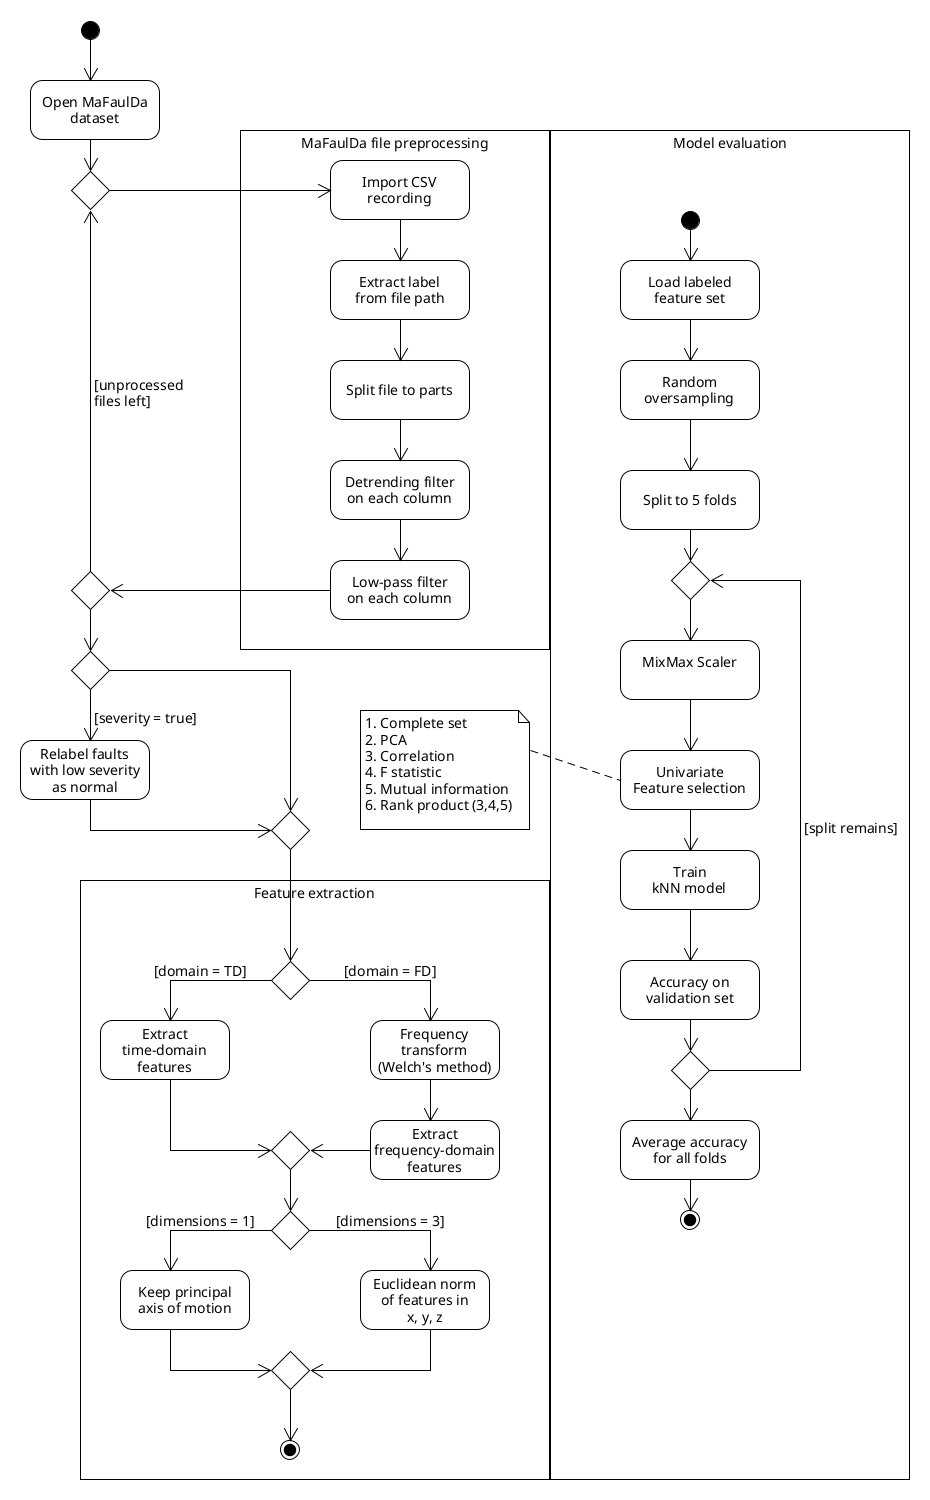
\includegraphics[width=0.9\textwidth]{assets/design/pipeline-design.png}
	\caption{Machine learning pipeline for MaFaulDa dataset}
	\label{fig:design:ml-pipeline}
\end{figure}
\afterpage{\clearpage}

\textbf{In preprocessing step}, the signals stored in columns of CSV files within the MaFaulDa ZIP archive are first associated with metadata according to the file's path in the directory structure. The hierarchically topmost folder describes the simulated defect. There is directory for \emph{normal}, \emph{imbalance}, \emph{horizontal-misalignment}, \emph{vertical-misalignment}, \emph{overhang} (outer bearing), \emph{underhang} (inner bearing). Each bearing has an additional folder layer for dividing bearing faults: \emph{ball\_fault}, \emph{cage\_fault}, \emph{outer\_race}. Each fault category except the normal class contains various fault severities with units of grams or millimeters. The severities in turn consist of individual files with different rpm speeds. 

We neglect the acceleration sensor orientation, therefore, the labels for shaft misalignment in vertical and horizontal directions are merged into the same group. In the end, that leaves \textbf{6 types of labels}: baseline, two shaft faults are imbalance and misalignment, and three bearing faults are cage fault, ball fault, and outer race fault.  

Depending on the chosen bearing position, only time series associated with that bearing are retained because the standards demand each bearing be assessed separately. Fault classification concerns bearing in direct contact and shaft mechanically passing through it.

The strength of the recorded response to the underlying defect is dependent on the shaft \textbf{rotational speed}. Speed in units of rpm is calculated from pulsed speedometer output. It is the average distance between two successive rising edges:
\begin{ceqn}\begin{align}
\mathrm{rpm} = 60 \;/\; \overline{\Delta t}
\end{align}\end{ceqn}

The final \textbf{file description} is the triplet of \textbf{fault}, \textbf{severity}, and \textbf{rpm}.

After labeling we insert a step to split the time series into parts when the duration is long enough to introduce more observations artificially. This assumption is not met for MaFaulDa because, for the desired frequency resolution for features of close to 1~Hz, we need a window size of 32768 samples. Variation reduction in spectral estimation brings the necessity to average at least 12 overlapping windows. The full length of 5 seconds provides 15 whole overlapping windows. 

The DC component in the three-dimensional vibration signal is removed by subtracting the global mean. Immediately follows a digital IIR Butterworth low pass filter of \nth{5} order with cutoff frequency 10 kHz at -3 dB. Before the usage of a low pass filter, the peak at 20 kHz with a sideband was present as an unwanted artifact. It could not have been reliably recorded due to the linear frequency response of the sensor up to 10 kHz. At the same time, such a frequency is outside the range of any feasible MEMS accelerometer.

Initial labels can be exchanged for a label of fault-free state when the severity is low. The count of severity levels is not identical in every group. The numerical amounts for each level are sorted in ascending order within each fault and then these levels are normalized using a min-max scaler.

The preprocessed signal from each axis of accelerometer is packed up to two base feature sets in time domain (TD) and frequency domain (FD). The feature extraction formulas are is identical with formulas presented in the section \ref{section:feature-extraction} of analysis chapter. The frequency transform is Welch's method averaging FFT vectors from 32768 samples after Hann windowing and 50\% overlap. The feature sets are:
\begin{itemize}
\itemsep0pt
\item \textbf{TD has 10 time-domain features} - peak-to-peak amplitude (\emph{pp}), zero-crossing rate (\emph{zerocross}), root mean square (\emph{rms}), skewness, kurtosis, shape factor, crest factor, impulse factor, clearance factor, average amplitude change (aac), 
\item \textbf{FD has 11 frequency-domain features} - spectral centroid, standard deviation (\emph{std}), skewness, kurtosis, roll-on frequency, roll-off frequency, spectral flux, noisiness, spectral negentropy, energy, entropy.
\end{itemize}
 
The four conditions are applied in the instance of the pipeline to filter observations with calculated features to create 24 scenarios:
\begin{itemize}
\itemsep0pt
\item \textbf{Source bearings} - samples and fault labels are left in either just for the inner bearing (A), for only the outer bearing (B), or for both bearings (A+B).
\item \textbf{Feature domain} - the set of extracted features as an input to downstream models is changed either to TD or FD set,
\item \textbf{Accelerometer axis} - Either one principal direction of motion or all three dimensions is aggregated under same feature name (1 or 3),
\item \textbf{High severity faults} - to more precisely simulate fault frequencies found in real environment the low severity defects can be considered as normal operation (Yes or No).
\end{itemize}

The fault classification performance metrics are evaluated after balancing classes feature normalization, and 5-fold cross-validation validation on the k-nearest neighbor classifier with Euclidean distance metric. The population of classes is evened out with random oversampling using a strategy to resample all but the majority class. In the multi-class classification, the micro-averaged performance metrics of accuracy, precision, and recall result in the same number. Therefore, accuracy is only one on the output. 

The hyperparameter of k-neighbours and a subset of features are tweaked, and results are compared under different preprocessing conditions and in multiple experiments:

\begin{itemize}
\itemsep0pt
\item \textbf{Complete feature sets}: compare the accuracy of the k-NN model in relation to the k-value as an odd number in the range from 1 to 37 on the dataset under different conditions. The TD and FD sets are treated separately.

\item \textbf{Feature combinations} - every combination of feature subsets with 2, 3, and 4 members are evaluated to obtain the statistical distribution of all possible k-NN models. The k-value is sequentially increased from options 3, 5, and 11 neighbours. The single k-value generates $\sum_{j=2}^{4}{\binom{n}{j}}$ where $n$ is number of members in complete feature set. In total 375 models for TD and 550 models for FD are tested under identical conditions. 

The observed effect is a rate of decrease in accuracy while shrinking the number of features to the bare minimum. The side product is finding the global optimum by brute force of the most informative attributes in predicting the defect.

\item \textbf{Feature selection methods} - the choice of feature subset is performed in linear time complexity as opposed to exponential in combinatorial case. The dimensionality reduction using \textbf{principal components analysis} (PCA) does further extraction and retains only the components that best explain the variance. The disadvantage is that the resulting linear combination cannot be interpreted easily. 

The best feature subset from complete sets is picked after ranking the features according to their importance. The bivariate scores for ranking are the mean of point biserial \textbf{correlation} to every class label as a dichotomous variable, \textbf{Fisher score} (F statistic), and \textbf{Mutual information}. The rank product combines the three latter scores into the ensemble. The comparison for the accuracy of the feature selection strategy is made in relation to the entire model accuracy distribution. 

\item \textbf{Incremental learning} - the order of samples tries to simulate the gradually worsening state of the machine and delayed annotation of defects. Observations are sorted based on increasing relative severity. The faults with the same severity are lined up randomly. 

The \textbf{tumbling window} of lengths 1, 10, 100 measurements imitates regular expert visits annotating observations recorded until that moment. Labels for the whole previous window are supplied at once.

Another common problem with online learning is \textbf{missing annotations} due to the size of the dataset. The equal-length gaps of 0, 2, 10, and 50 labels are skipped before another observation is annotated. This approach of skipping samples without considering their representativeness can result in harm to predictions. 
\end{itemize}

The experimental design involves the filter conditions that create 24 forms of the original MaFaulDa. The four main experiments test hyperparameters on each dataset variation. Those are k-neighbors, a number and kind of features in batch learning tumbling windows, and label skips in incremental learning.

\section{Exploratory data analysis of MaFaulDa}
% To better explain the behavior of the models we examine number of observation per fault category and spatial separability of the groups, ranges and interdependecies of the features. 

% Out of 1951 time series, just xx is for inner bearing (A) and xx for outer bearing. We can see taht by merging the vertical and horizontal misalignment this label has the most occurence with xx\%. Normal class is the less populous with just xx\%.
\begin{table}[h]
\renewcommand{\arraystretch}{1.2}
\centering
\begin{tabular}{|lr|r|r|r|r|r|r|}
\hline
\multicolumn{2}{|l|}{\textbf{Bearing}}                                            & \multicolumn{1}{l|}{A}  & \multicolumn{1}{l|}{A+B} & \multicolumn{1}{l|}{B}  & \multicolumn{1}{l|}{A}   & \multicolumn{1}{l|}{A+B} & \multicolumn{1}{l|}{B}   \\ \hline
\multicolumn{2}{|l|}{\textbf{Relabel by severity}}                                & \multicolumn{1}{l|}{No} & \multicolumn{1}{l|}{No}  & \multicolumn{1}{l|}{No} & \multicolumn{1}{l|}{Yes} & \multicolumn{1}{l|}{Yes} & \multicolumn{1}{l|}{Yes} \\ \hline
\multicolumn{1}{|l|}{\multirow{6}{*}{\textbf{Fault}}} & \textbf{misalignment}     & 498                     & 996                      & 498                     & 248                      & 496                      & 248                      \\ \cline{2-8} 
\multicolumn{1}{|l|}{}                                & \textbf{imbalance}        & 333                     & 666                      & 333                     & 188                      & 376                      & 188                      \\ \cline{2-8} 
\multicolumn{1}{|l|}{}                                & \textbf{cage fault}       & 188                     & 376                      & 188                     & 91                       & 181                      & 90                       \\ \cline{2-8} 
\multicolumn{1}{|l|}{}                                & \textbf{ball fault}       & 186                     & 323                      & 137                     & 87                       & 132                      & 45                       \\ \cline{2-8} 
\multicolumn{1}{|l|}{}                                & \textbf{outer race fault} & 184                     & 372                      & 188                     & 86                       & 176                      & 90                       \\ \cline{2-8} 
\multicolumn{1}{|l|}{}                                & \textbf{normal}           & 49                      & 98                       & 49                      & 738                      & 1470                     & 732                      \\ \hline
\multicolumn{2}{|l|}{$\Sigma$}                                                    & \textbf{1438}           & \textbf{2831}            & \textbf{1393}           & \textbf{1438}            & \textbf{2831}            & \textbf{1393}            \\ \hline
\end{tabular}
\caption{Number of rows in MaFaulDa according to label}
\end{table}

% The inner and outer bearings each have diffent number of recodings made so the total counts differ: xx for bearing A and xx for bearing B. After relabeling the normal class became the largest taking up xx\%. Bearing A+B just concatanes observations from both beraings so the value is the sum. Inbalance ratio as a largest to smallest numbered class is xx \% for original labels and xx \% after relabeling

% Correlation to RPM
\begin{figure}[h]
    \centering
    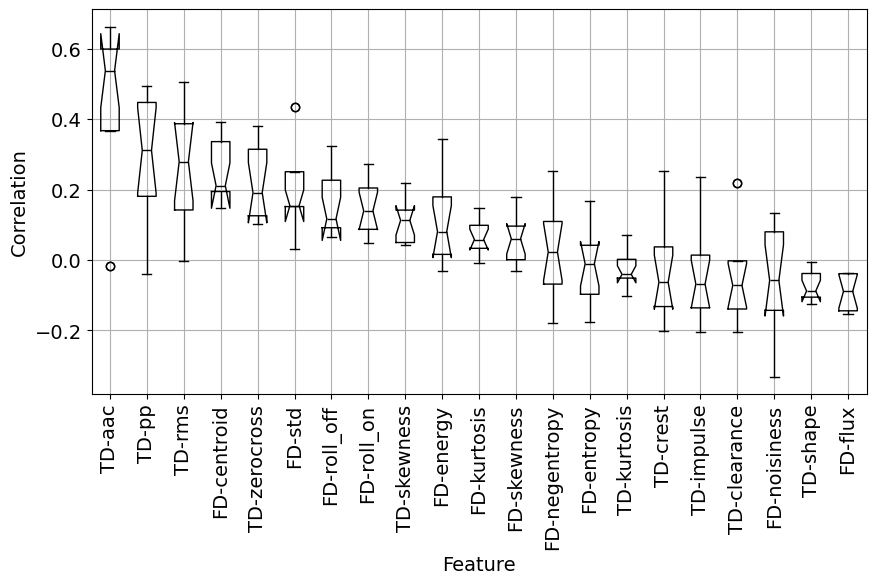
\includegraphics[width=\textwidth]{assets/results/feature-values/corr-to-rpm.png}
    \caption{Correlation of features to RPM over all experiments}
\end{figure}

% Feature correlations
\begin{figure}[h]
    \centering
    \begin{subfigure}[b]{0.48\textwidth}
        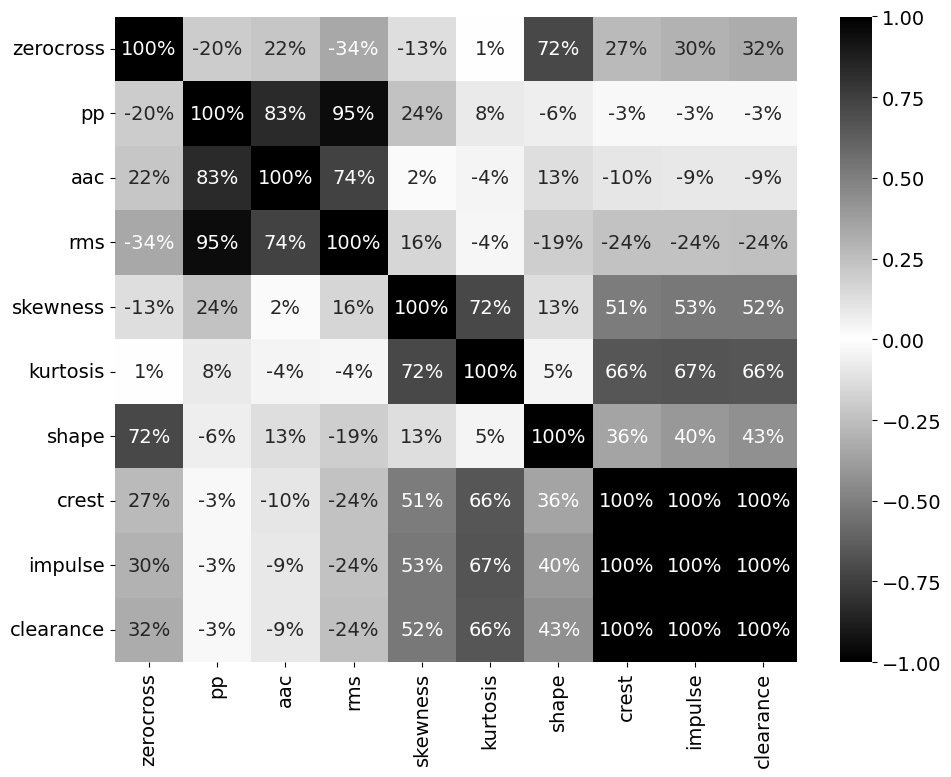
\includegraphics[width=\textwidth]{assets/results/feature-values/corr-A-3-TD.png}
        \caption{Time-domain features}
    \end{subfigure}
    \hfill
    \begin{subfigure}[b]{0.48\textwidth}
        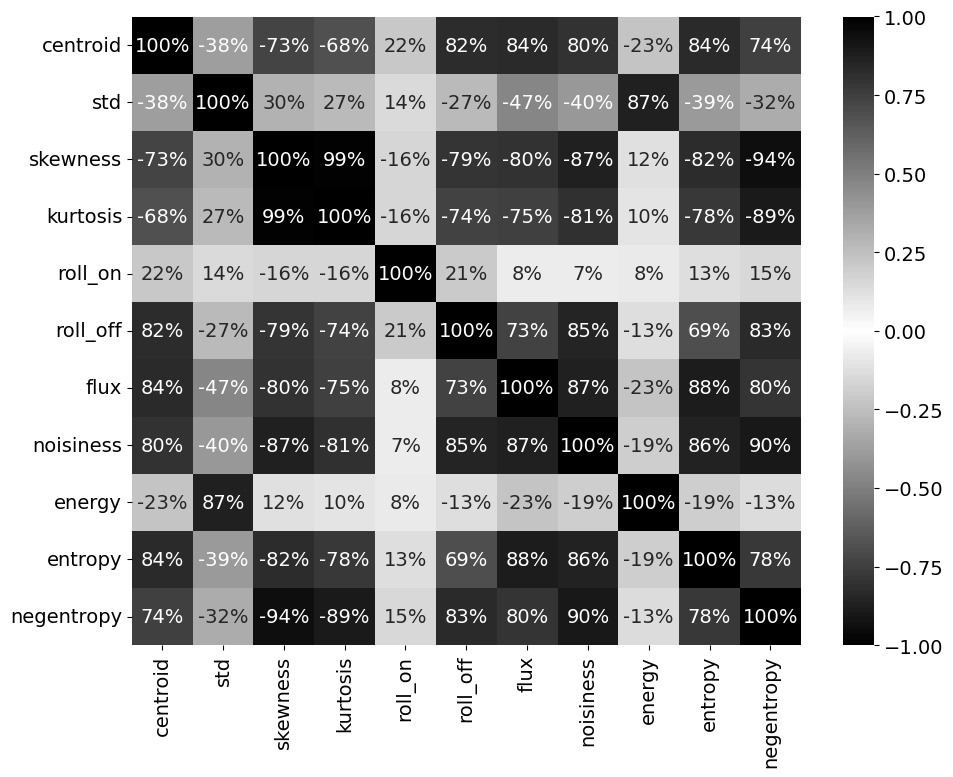
\includegraphics[width=\textwidth]{assets/results/feature-values/corr-A-3-FD.png}
        \caption{Frequency-domain features}
    \end{subfigure}
    \caption{Feature correlations in MaFaulDa}
\end{figure}


% Features Range
% Mafaulda
\begin{figure}[h]
    \centering
    \begin{subfigure}[b]{0.48\textwidth}
        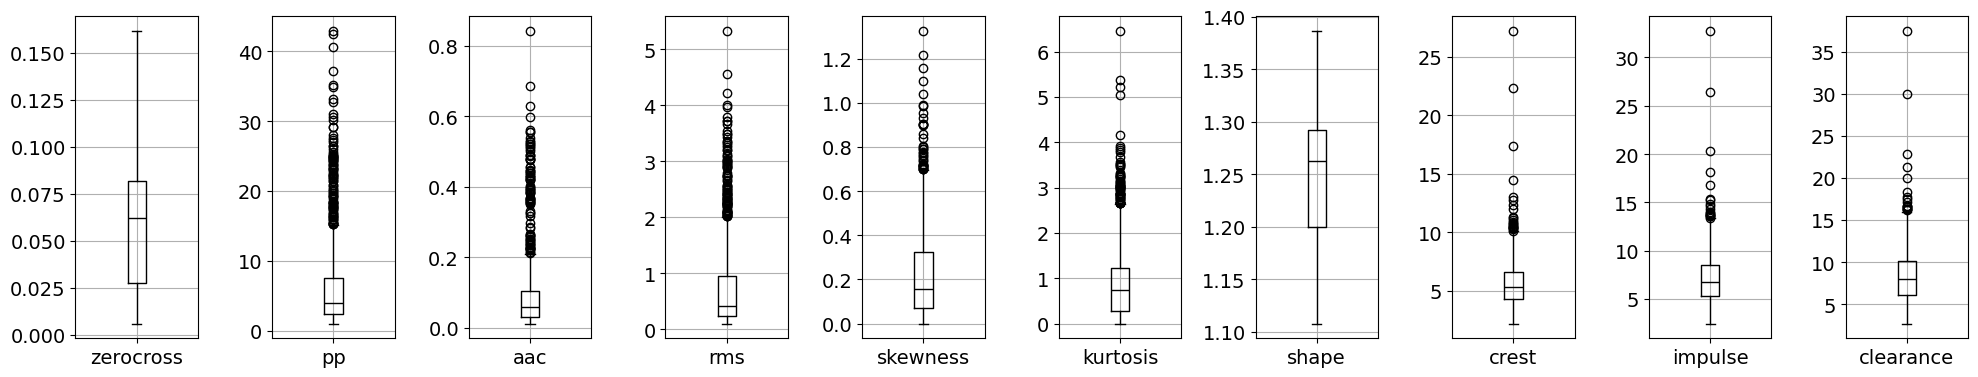
\includegraphics[width=\textwidth]{assets/results/feature-values/features-TD-dim1-A.png}
        \caption{Time-domain features}
    \end{subfigure}
    \hfill
    \begin{subfigure}[b]{0.48\textwidth}
        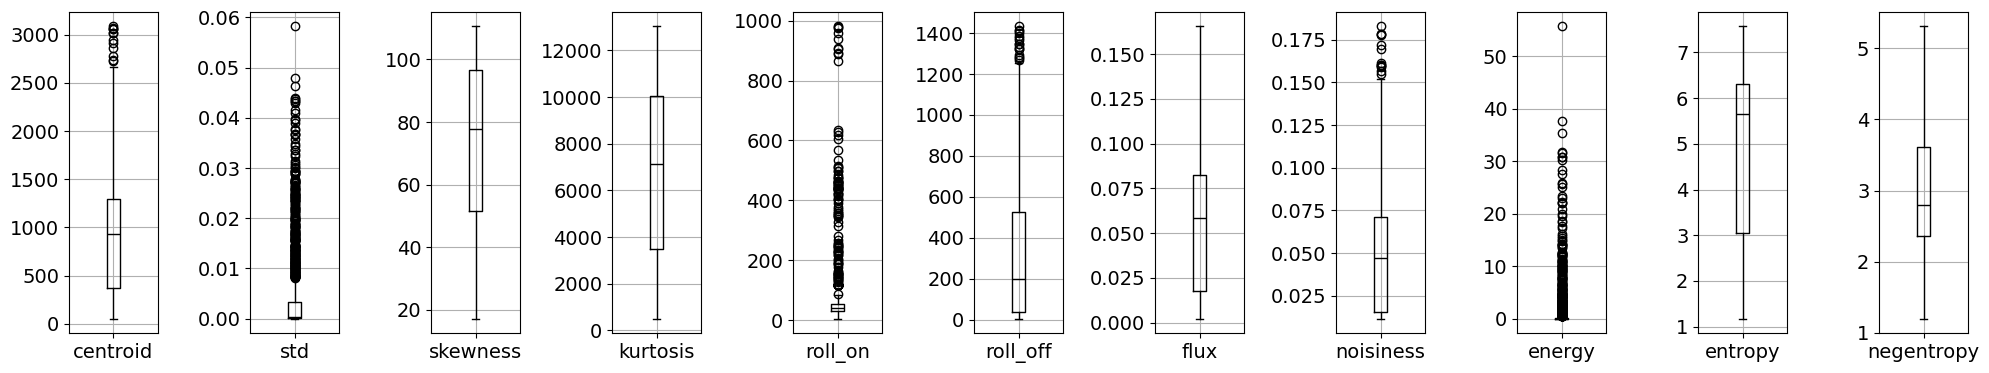
\includegraphics[width=\textwidth]{assets/results/feature-values/features-FD-dim1-A.png}
        \caption{Frequency-domain features}
    \end{subfigure}
    \begin{subfigure}[b]{0.48\textwidth}
        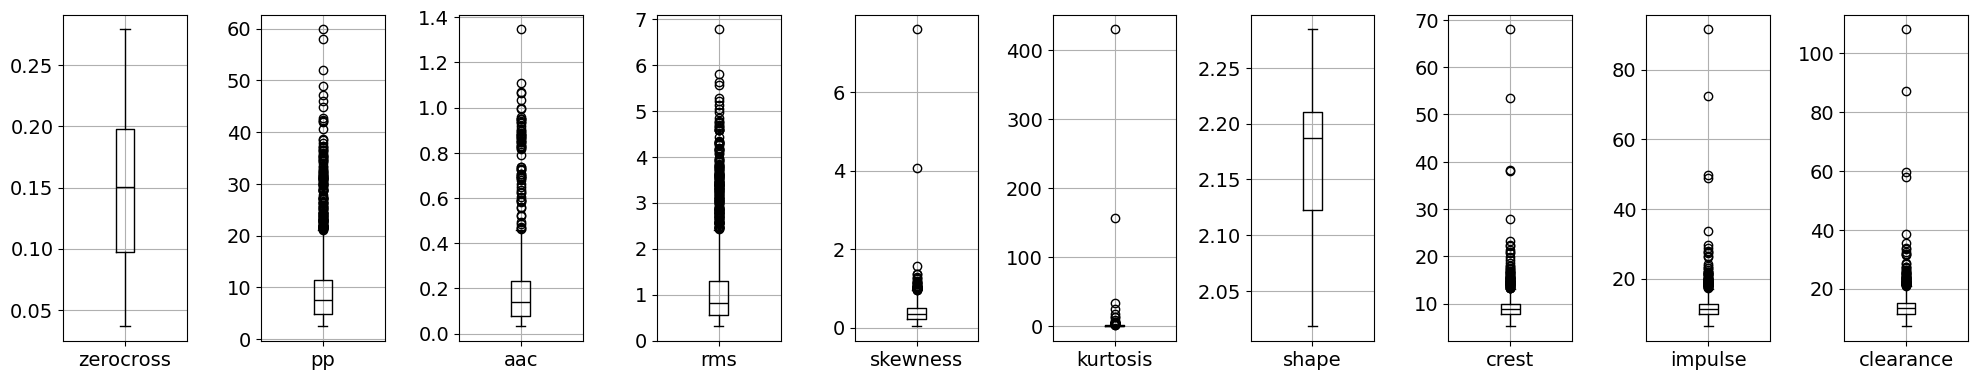
\includegraphics[width=\textwidth]{assets/results/feature-values/features-TD-dim3-A.png}
        \caption{Time-domain features}
    \end{subfigure}
    \hfill
    \begin{subfigure}[b]{0.48\textwidth}
        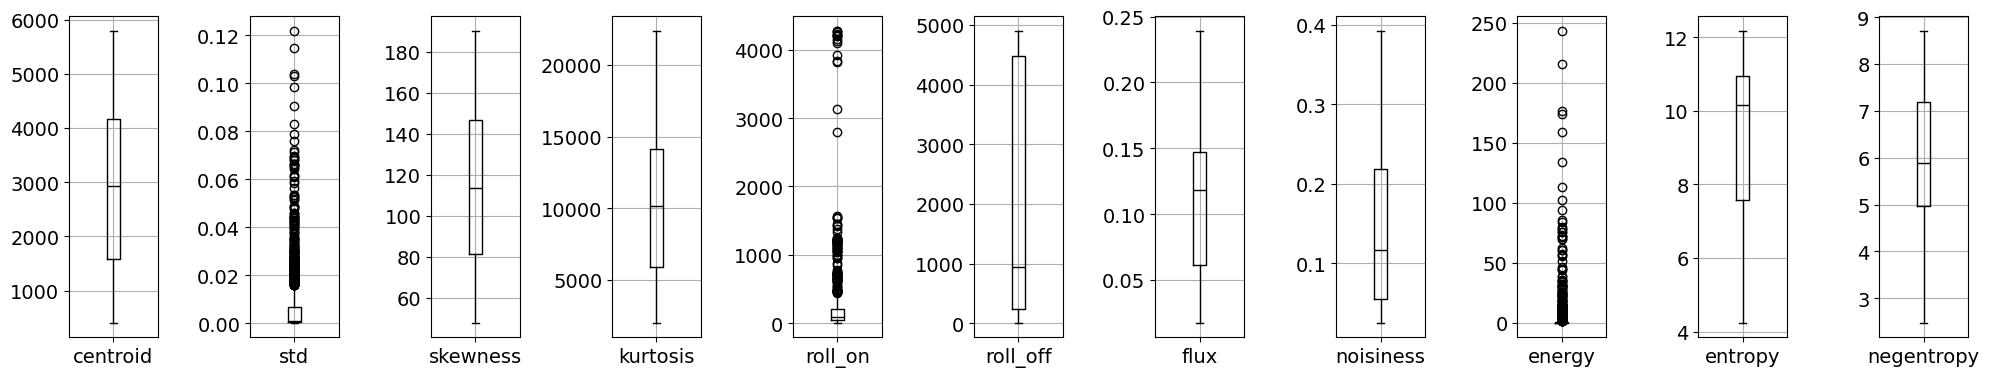
\includegraphics[width=\textwidth]{assets/results/feature-values/features-FD-dim3-A.png}
        \caption{Frequency-domain features}
    \end{subfigure}
    \caption{Feature range in MaFaulDa}
\end{figure}

% PCA plot of labels
% Clusters with true labels
\begin{figure}[h]
    \centering
    \begin{subfigure}[b]{0.48\textwidth}
        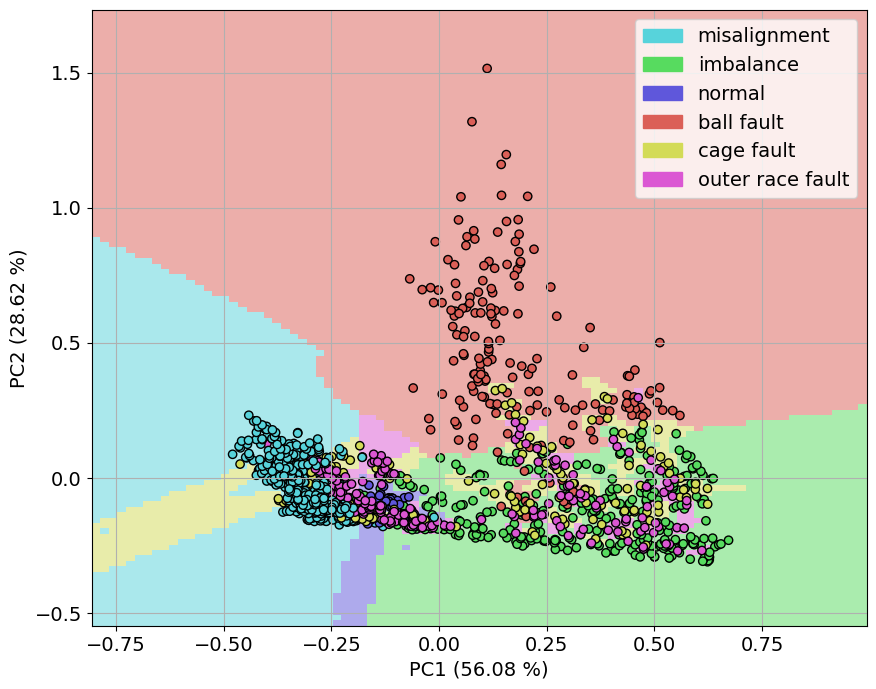
\includegraphics[width=\textwidth]{assets/results/labels/PCA-TD.png}
        \caption{Time-domain features}
    \end{subfigure}
    \hfill
    \begin{subfigure}[b]{0.48\textwidth}
        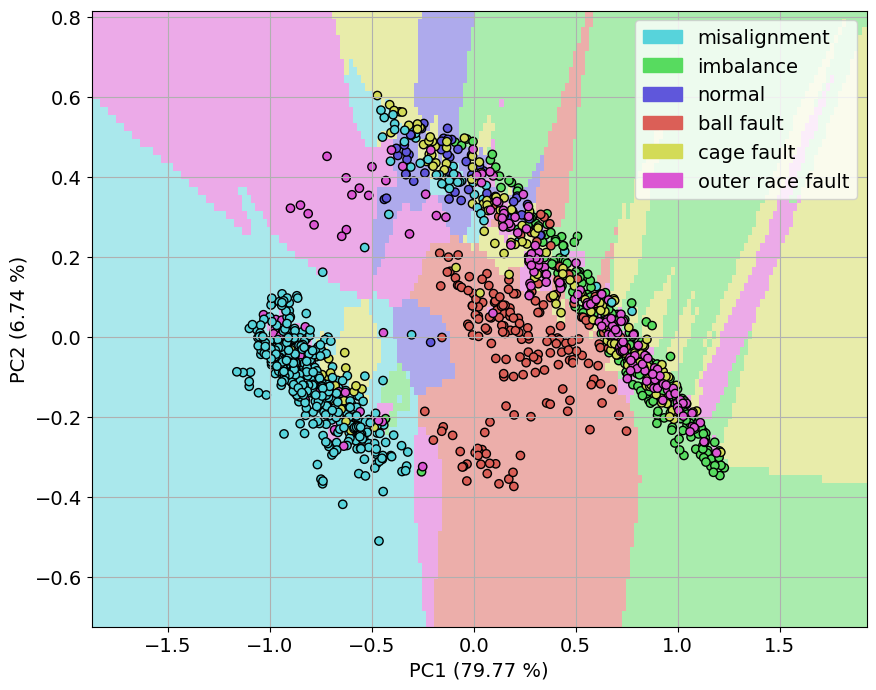
\includegraphics[width=\textwidth]{assets/results/labels/PCA-FD.png}
        \caption{Frequency-domain features}
    \end{subfigure}
    \hfill
    \begin{subfigure}[b]{0.48\textwidth}
        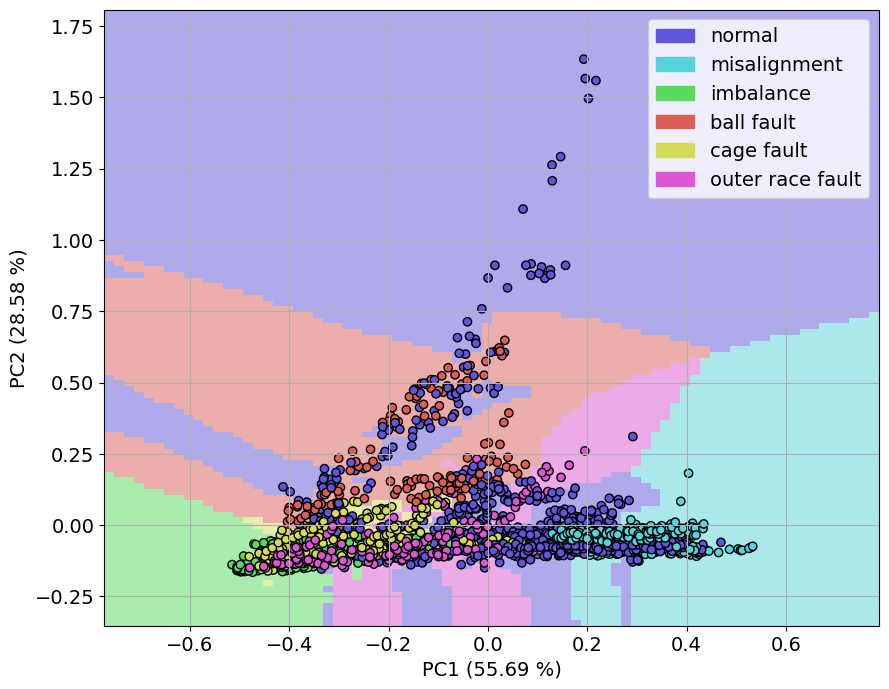
\includegraphics[width=\textwidth]{assets/results/labels/PCA-TD-severity.png}
        \caption{Time-domain features (severity)}
    \end{subfigure}
    \hfill
    \begin{subfigure}[b]{0.48\textwidth}
        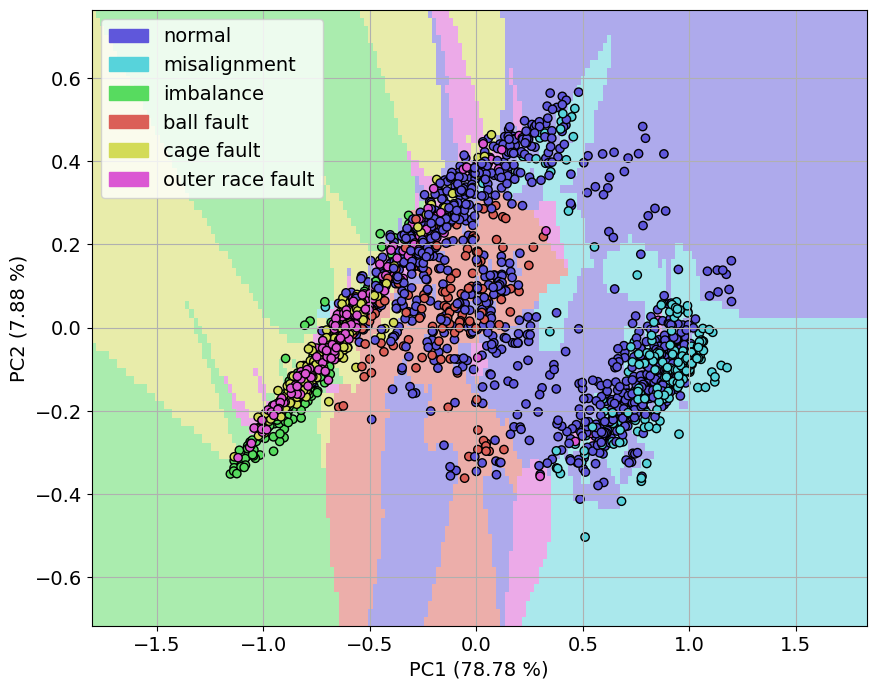
\includegraphics[width=\textwidth]{assets/results/labels/PCA-FD-severity.png}
        \caption{Frequency-domain features (severity)}
    \end{subfigure} 
    \caption{PCA of all features to 2 components}
\end{figure}

% Time domain waveforms of different faults
\begin{figure}[h]
    \centering
    \begin{subfigure}[b]{0.49\textwidth}
        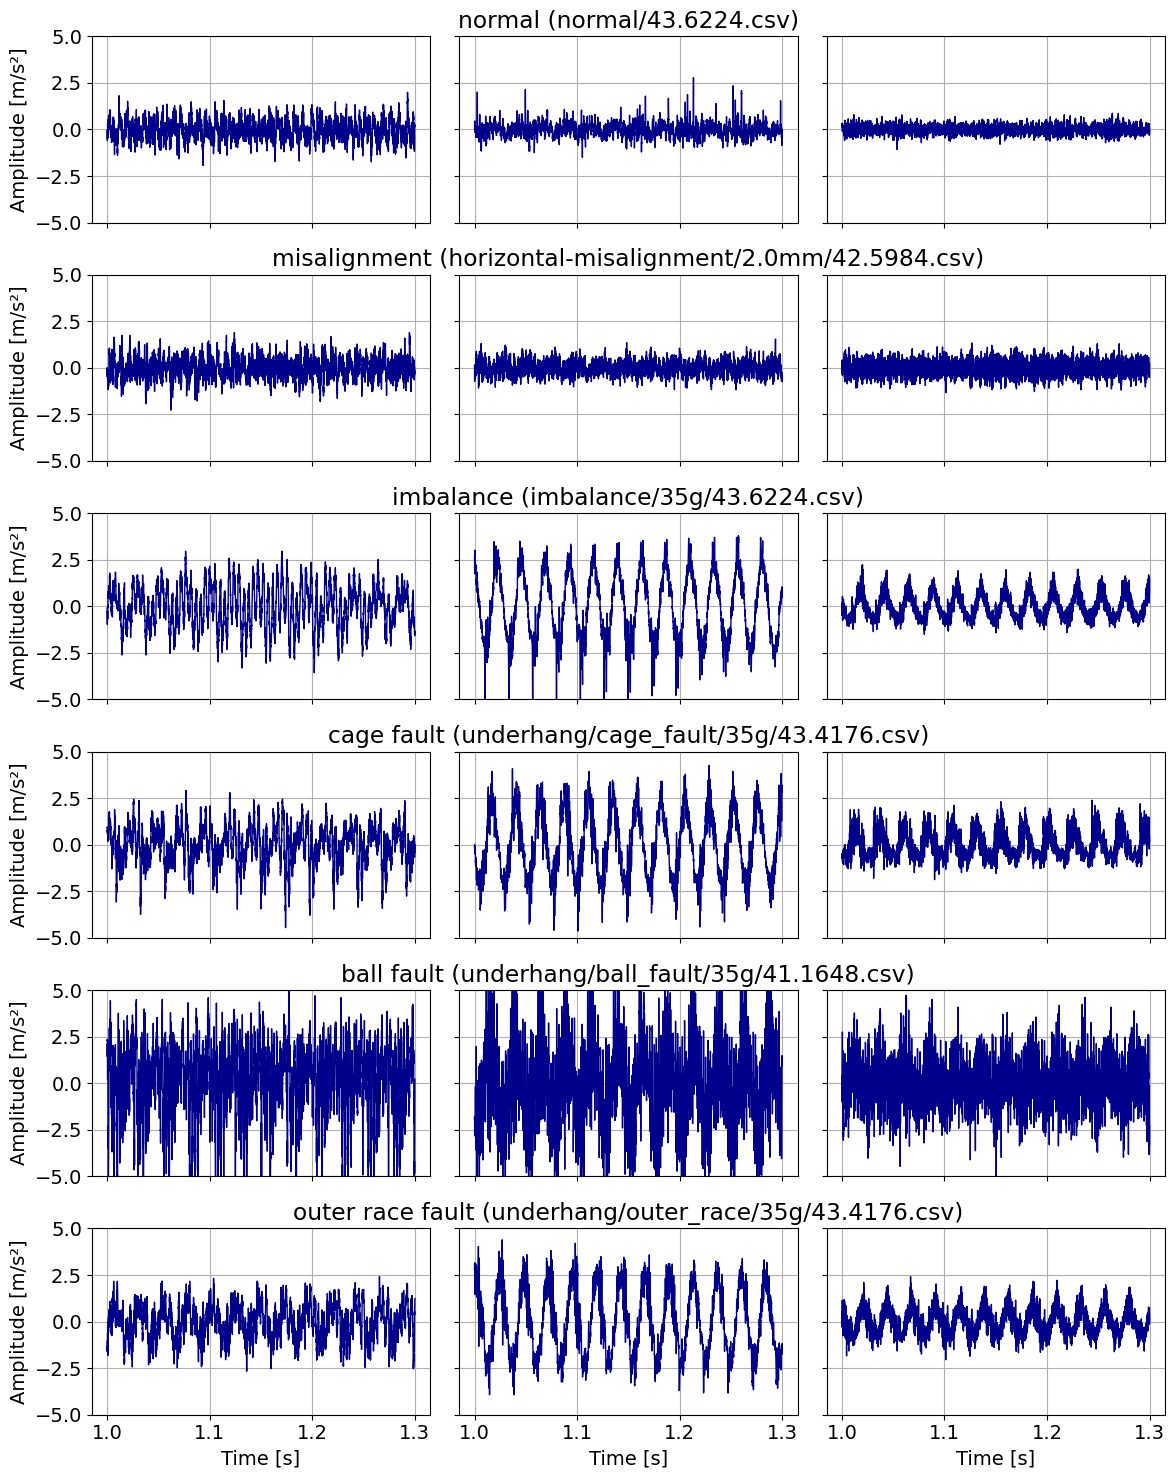
\includegraphics[width=\textwidth]{assets/results/eda/mafaulda-TD-A.png}
        \caption{Time domain}
    \end{subfigure}
    \hfill
    \begin{subfigure}[b]{0.49\textwidth}
        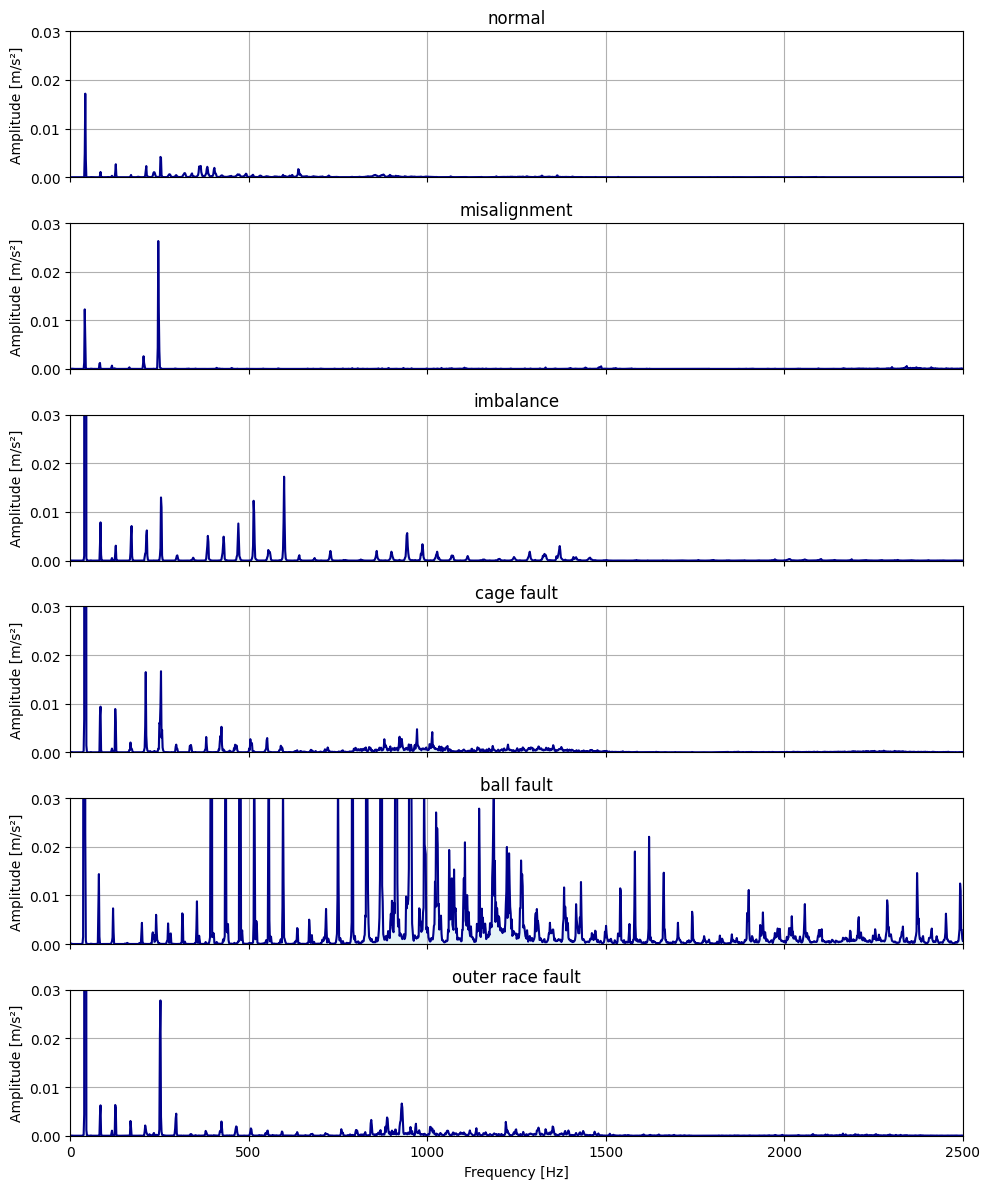
\includegraphics[width=\textwidth]{assets/results/eda/mafaulda-faults.png}
        \caption{Frequency domain (around 2500 rpm)}
    \end{subfigure}
    \caption{MaFaulDa}
\end{figure}


% PCA loading plots
\begin{figure}[h]
    \centering
    \begin{subfigure}[b]{\textwidth}
        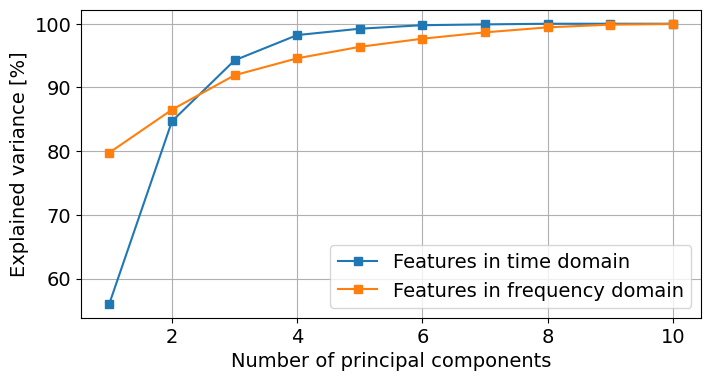
\includegraphics[width=\textwidth]{assets/results/eda/PCA-explained-variance.png}
        \caption{Time-domain features}
    \end{subfigure}
    \hfill
    \begin{subfigure}[b]{0.48\textwidth}
        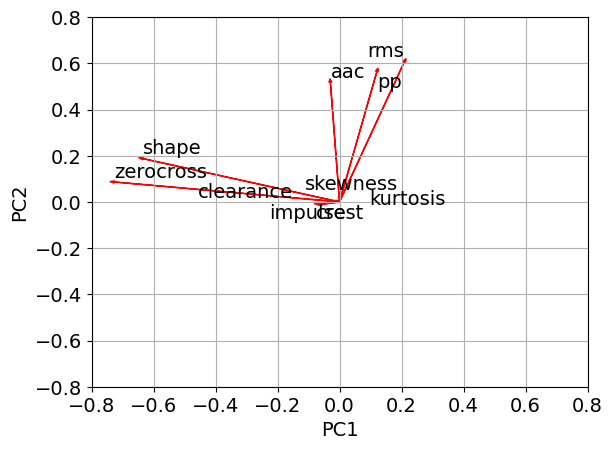
\includegraphics[width=\textwidth]{assets/results/eda/PCA-TD-loading-plot.png}
        \caption{Frequency-domain features}
    \end{subfigure}
    \hfill
    \begin{subfigure}[b]{0.48\textwidth}
        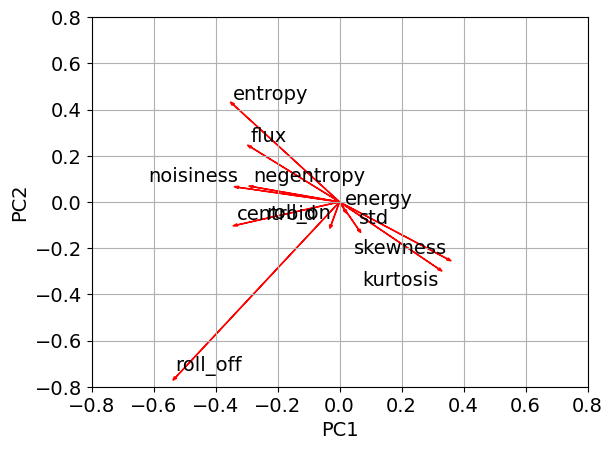
\includegraphics[width=\textwidth]{assets/results/eda/PCA-FD-loading-plot.png}
        \caption{Time-domain features (severity)}
    \end{subfigure} 
    \caption{PCA explained variance and loading plots (A bearing)}
\end{figure}

% silhouette score



\section{Accelerometer data logger}
% Block diagram of device

% HW parameters and mention temporary device
\begin{table}[h]
\renewcommand{\arraystretch}{1.2}
\centering
\begin{tabular}{|l|l|l|}
\hline
\textbf{Accelerometer}                           & \textbf{IIS3DWB}   \\ \hline
\textbf{Vendor}                                  & STMicroelectronics \\ \hline
\textbf{Bus}                                     & SPI                \\ \hline
\textbf{Axis}                                    & 1 or 3             \\ \hline
\textbf{Range} (g)                               & $\pm$ 2 - 16      \\ \hline
\textbf{Bandwidth} (kHz)                          & 5 - 6.3            \\ \hline
\textbf{Sensitivity} (mg/LSB)                    & 0.06 - 0.49       \\ \hline
\textbf{Noise density} ($\mu g / \sqrt{\mathrm{Hz}}$ rms) & 75                 \\ \hline
\textbf{Microcontroller}                         & ESP32-PoE-ISO      \\ \hline
\textbf{CPU SoC}                                 & ESP32-WROOM-32     \\ \hline
\textbf{Output data rate} (kHz)                  & 26.7               \\ \hline
\textbf{ADC resolution} (bit)                    & 16                 \\ \hline
\textbf{FIFO}                                    & 3 kB (512 samples) \\ \hline
\end{tabular}
\caption{Hardware parameters of accelerometer data logger}
\label{tab:design:hw-sensors}
\end{table}

\begin{figure}[h]
	\centering
	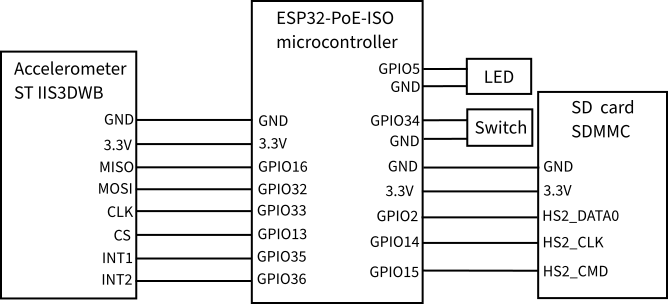
\includegraphics[width=0.9\textwidth]{assets/design/hw-block-schematic.png}
	\caption{Sensor unit hardware block diagram}
	\label{fig:design:block-diagram-hw}
\end{figure}

% Task communication sequence diagram

% Firmware
% Timing is crutial 19ms.
Activity diagrams describe three basic actions of firmware for logging accelerometer samples:

\begin{itemize}
\itemsep0pt
\item begin new recording, 
\item log block of samples into CSV file,
\item finish recording.
\end{itemize}

\begin{figure}[h]
    \centering
	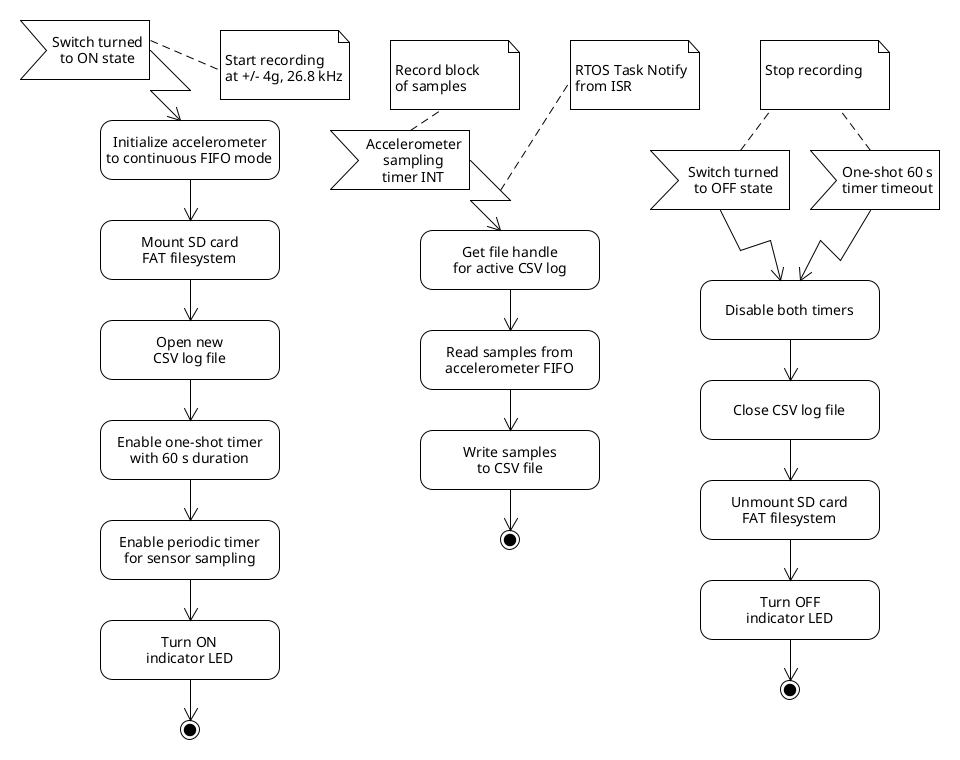
\includegraphics[width=\textwidth]{assets/design/firmware-design.png}
\end{figure} 


\section{Industrial equipment}
Three kinds of rotating machines are at disposal for vibration measurements. Those are a standing fan, scroll compressor, and water pump.

\begin{figure}[ht]
    \centering
    \begin{subfigure}[b]{0.17\textwidth}
    		\centering
        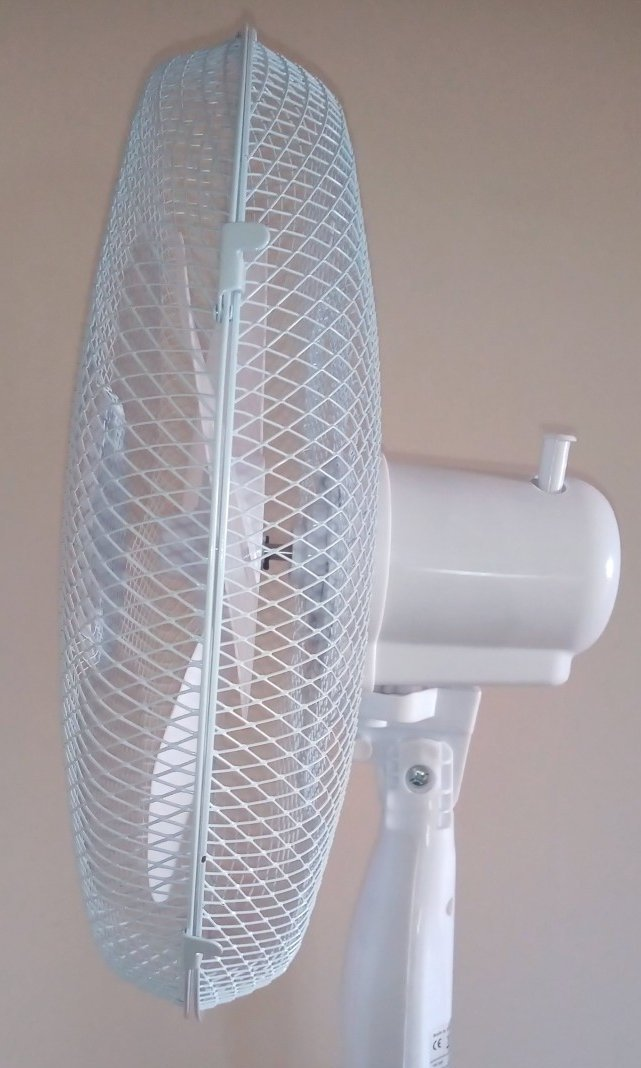
\includegraphics[width=\textwidth]{assets/design/machine-fan.jpg}
        \caption{\footnotesize Fan}
        \label{fig:machine:fan}
    \end{subfigure}
    \hfill
    \begin{subfigure}[b]{0.25\textwidth}
    		\centering
        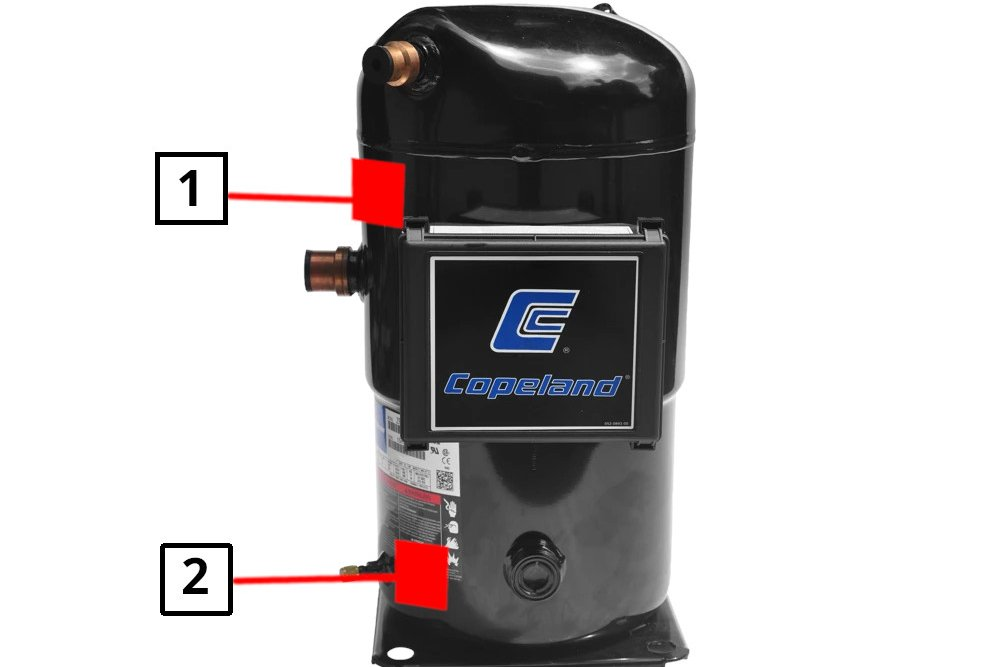
\includegraphics[width=\textwidth]{assets/design/sensor/copeland-compressor.jpg}
        \caption{\footnotesize Compressor}
        \label{fig:machine:compressor}
    \end{subfigure}
    \hfill
    \begin{subfigure}[b]{0.31\textwidth}
    		\centering
        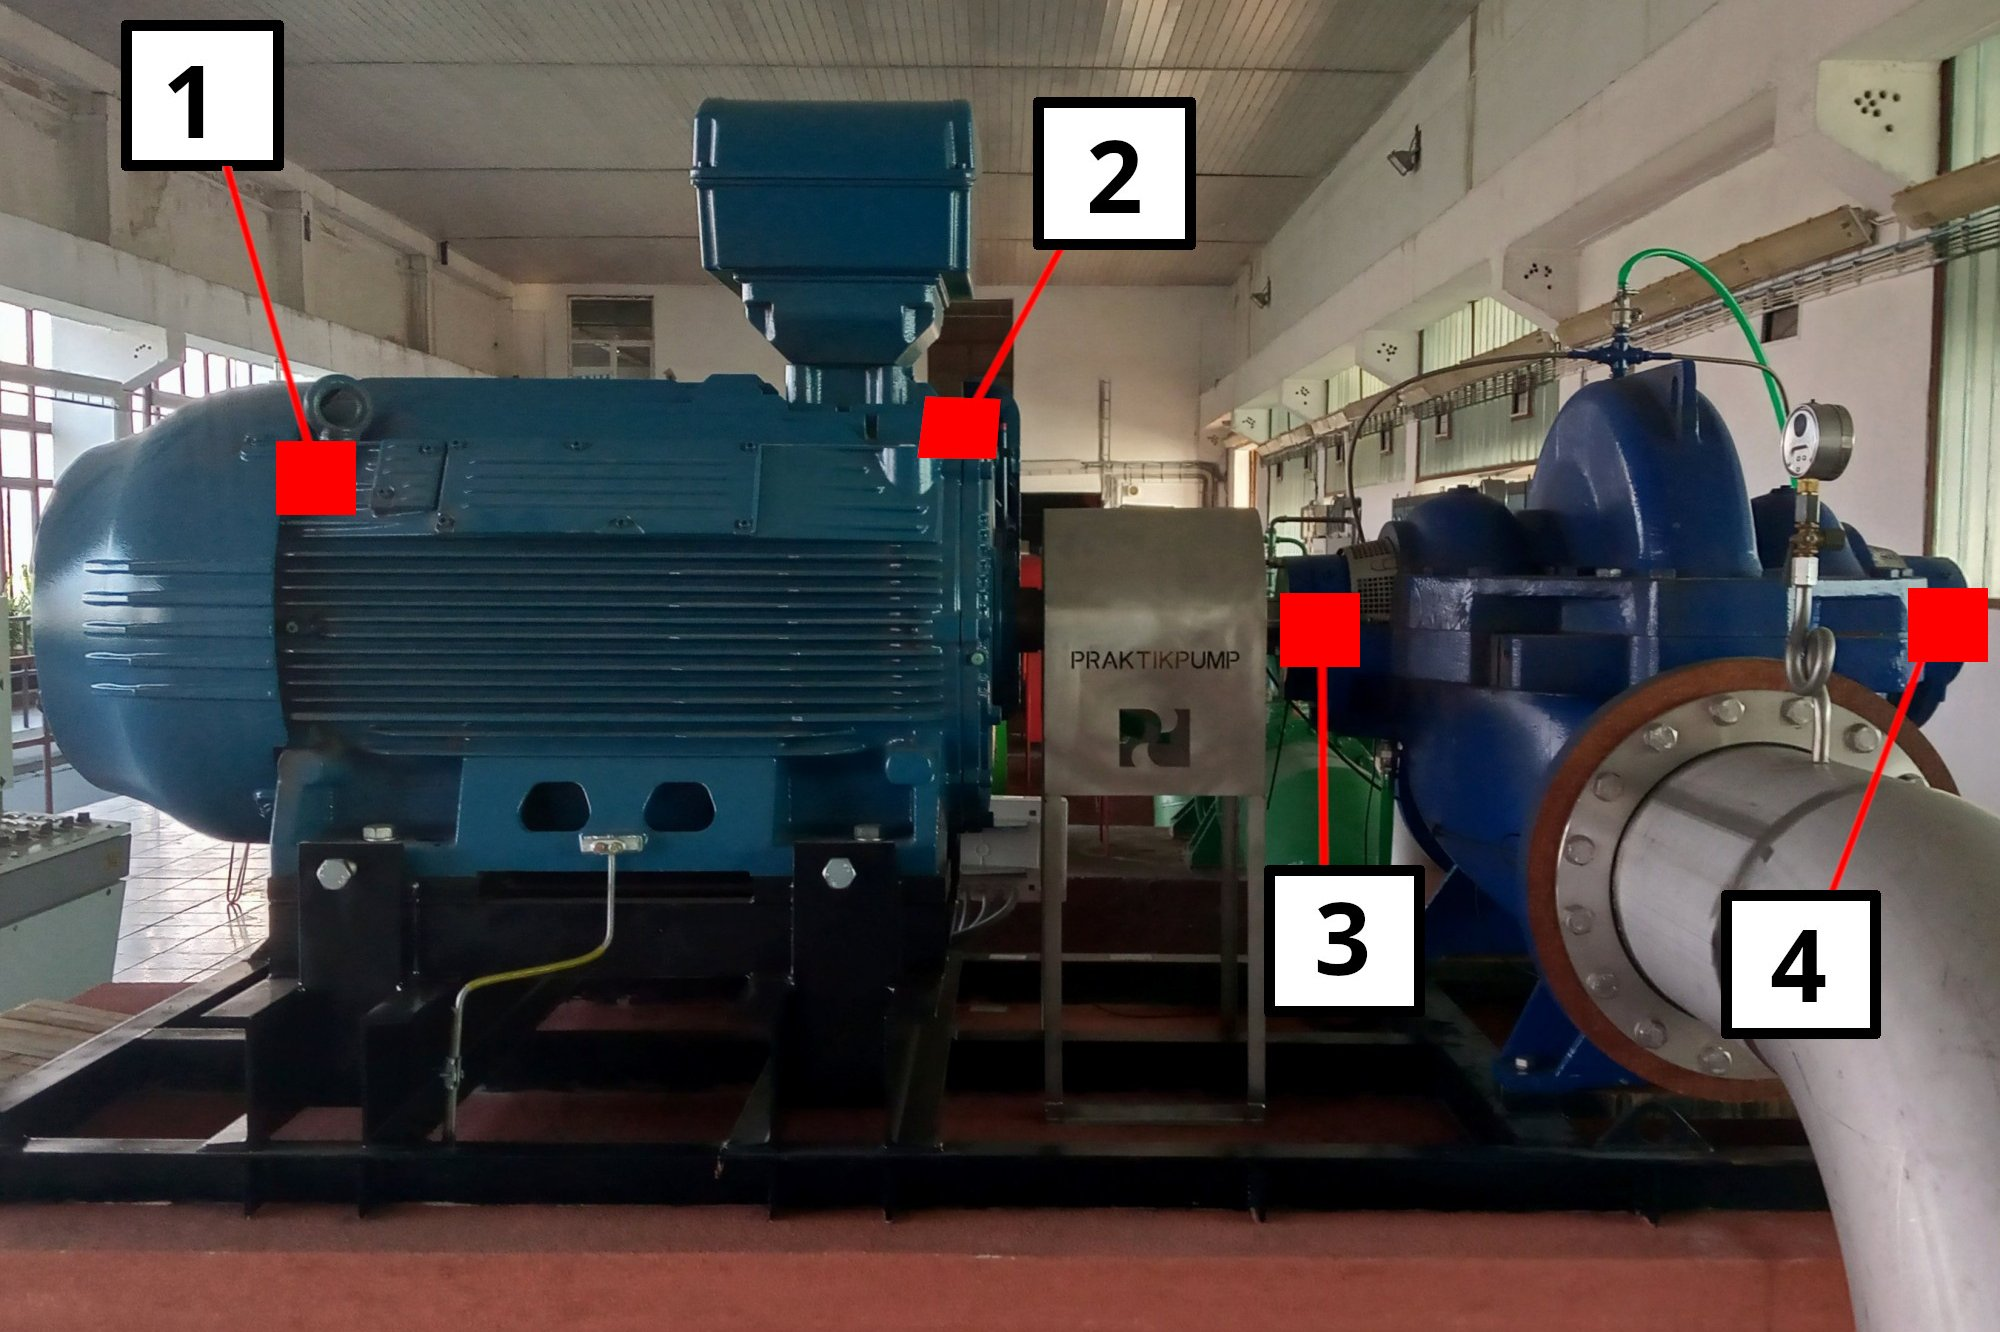
\includegraphics[width=\textwidth]{assets/design/sensor/ksb-pump.jpg}
        \caption{\footnotesize Water pump KSB}
        \label{fig:machine:pump-ksb}
    \end{subfigure}
    \hfill
    \begin{subfigure}[b]{0.31\textwidth}
    		\centering
        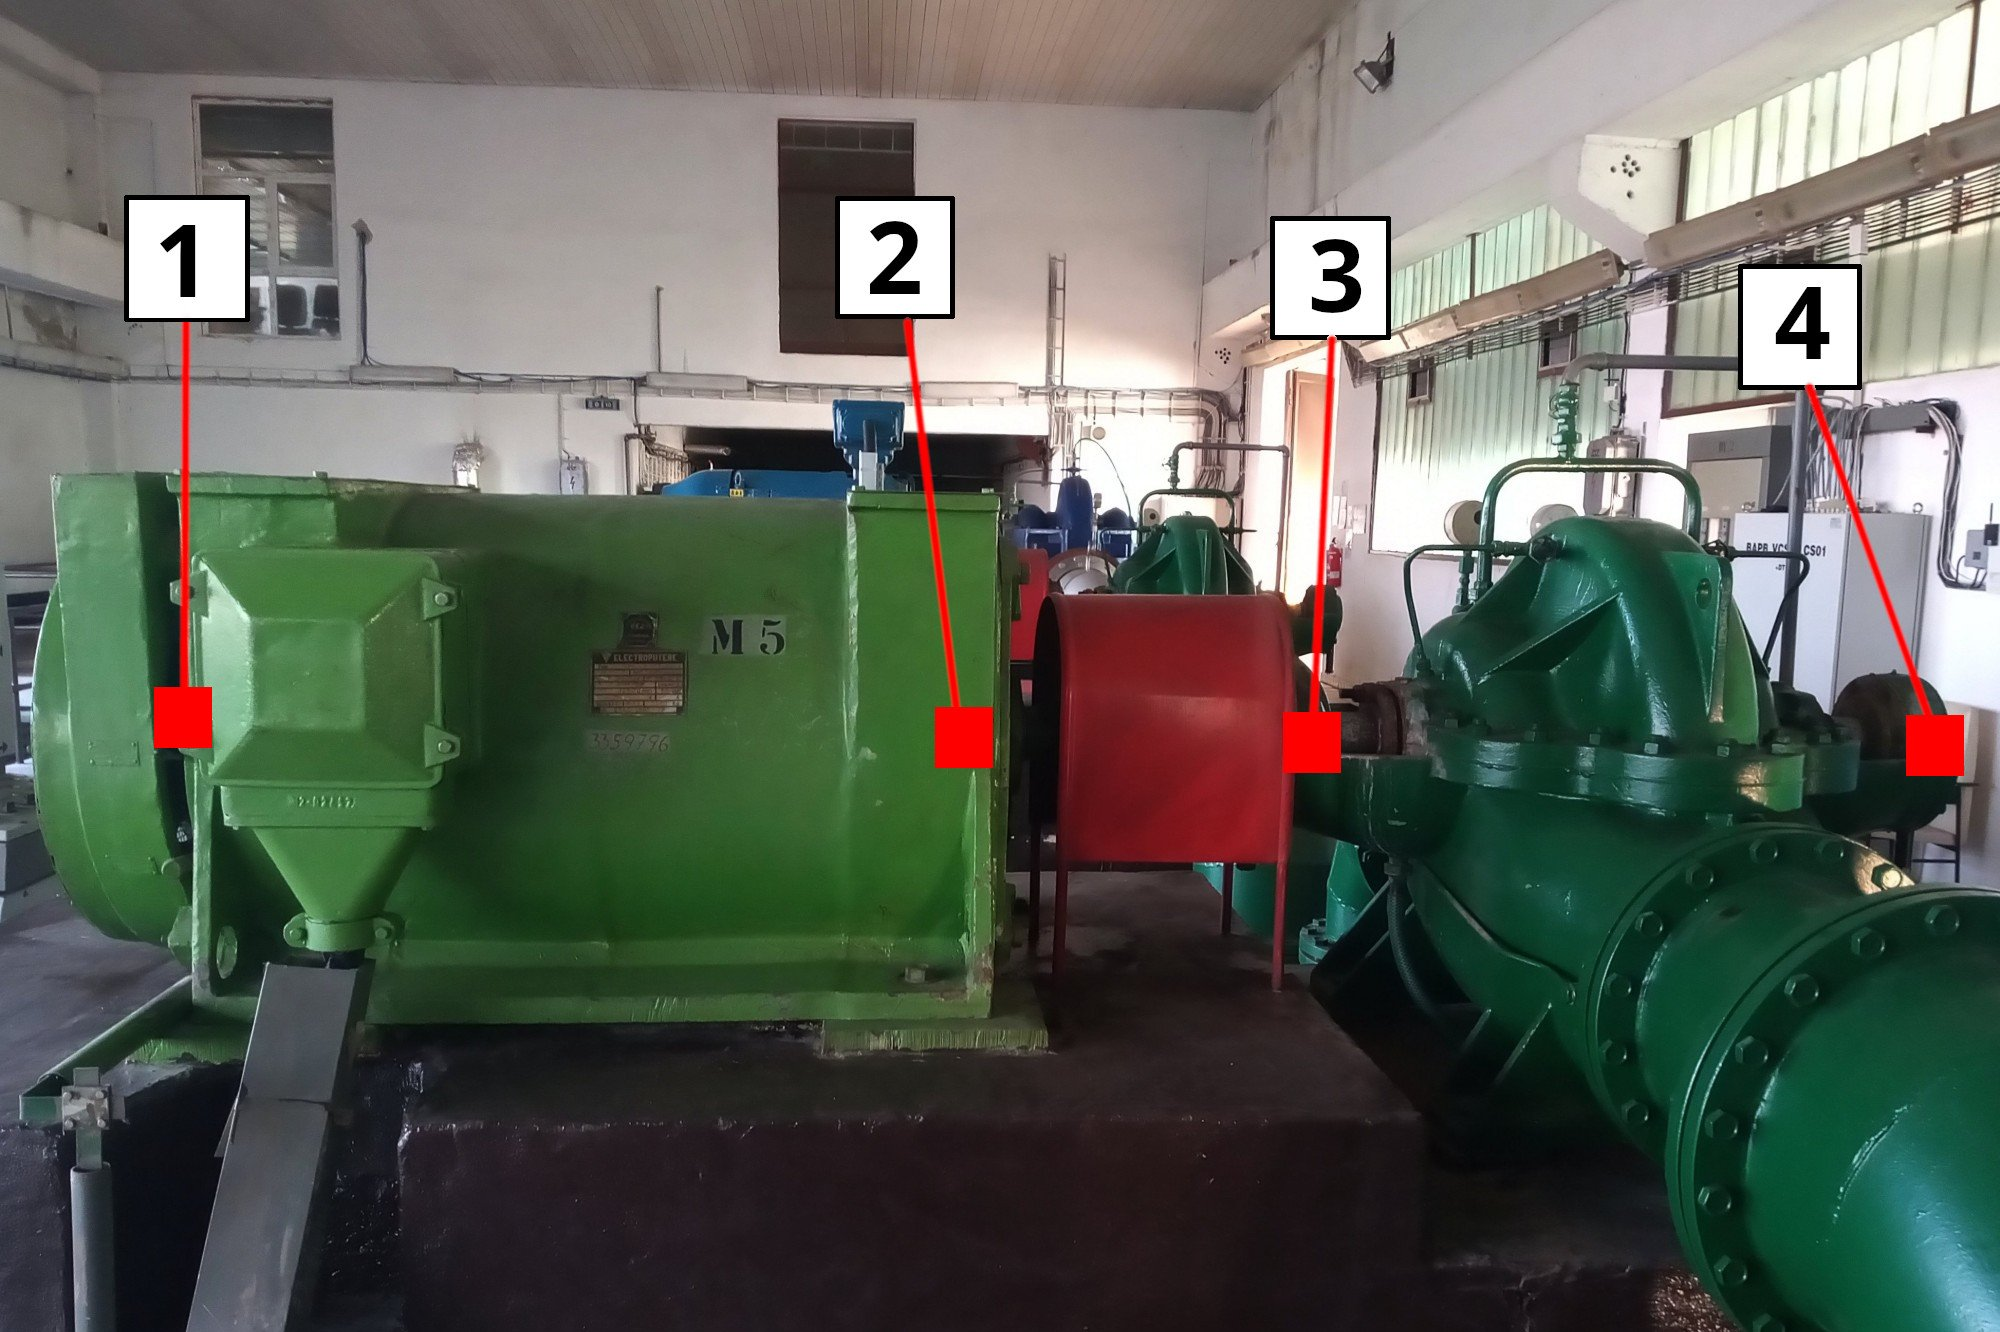
\includegraphics[width=\textwidth]{assets/design/sensor/sigma-pump.jpg}
        \caption{\footnotesize Water pump Sigma}
        \label{fig:machine:pump-sigma}
    \end{subfigure}
    \caption{Machines dedicated for vibration measurements}
\end{figure}

\textbf{Standing fan} is model \emph{Kalorik~TKG~VT1037} (Fig.~\ref{fig:machine:fan}) and one unit is available to us. It serves as a test bed during the sensor unit development. The sensor is placed on the plastic casing at the back of the drive motor. The fan has a 45~cm diameter with 3~propellers and a power of 45~W (class~\rom{1}). It has a switch for 3 rotational speeds, which are approximately 18.5~Hz (1100~rpm), 20.4~Hz (1200~rpm), and 22~Hz (1300~rpm).

\textbf{Scroll compressor} is model \emph{Copeland~ZR16} (Fig.~\ref{fig:machine:compressor}). Altogether, two units are available in two independent air conditioning units for the data center. The compressor has 9.7~kW of power (class~\rom{1}) and rotates at 2900 rpm (48.3 Hz). Two possible measurement locations are located on the sides on top of the bearings, just above the base and above the scroll.

\textbf{Water pumps} are available as 3 units in municipal drinking water pumping station. The apparatus consists of a single-stage axially split volute casing pump and an attached electric induction motor. 

The newer primary pumps with bundled wireless cloud monitoring system are two units of \emph{KSB Omega~300-560} (Fig.~\ref{fig:machine:pump-ksb}). The pumps were commissioned in 2018, and they rotate at 1493 rpm (24.9 Hz). The electric motor provides 400~kW of power (class~\rom{3}).

The secondary pump is one unit named \emph{Sigma~300-OVD-600} (Fig.~\ref{fig:machine:pump-sigma}) installed in 1986. It rotates at 1485 rpm (24.75 Hz), and its electric motor has power of 450~kW (class~\rom{3}). Each pump and motor have 2 bearings. Therefore, there are 4 measurement positions in total.

\begin{figure}[h]
    \centering
    \begin{subfigure}[b]{0.49\textwidth}
    		\centering
        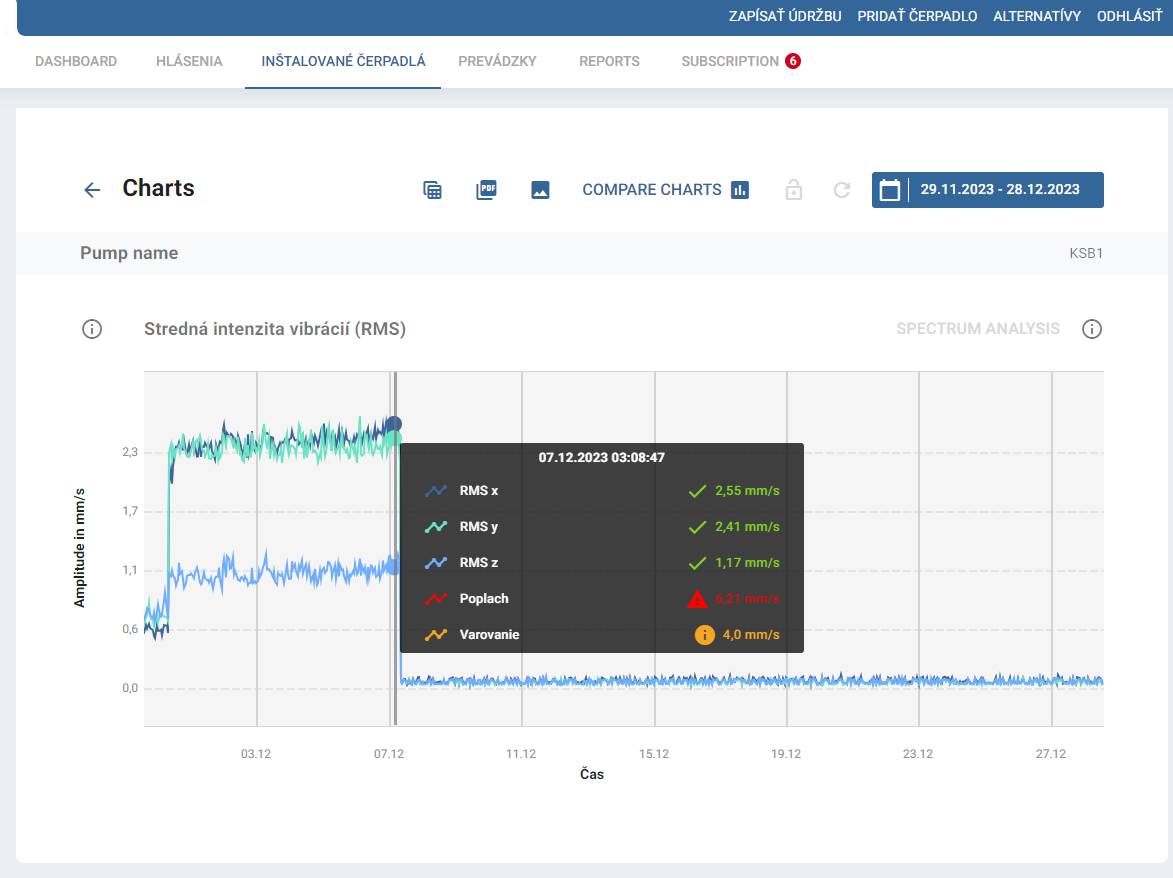
\includegraphics[width=\textwidth]{assets/design/ksb-guard-rms.png}
        \caption{Vibration rms velocity dashboard}
    \end{subfigure}
    \hfill
    \begin{subfigure}[b]{0.49\textwidth}
    		\centering
        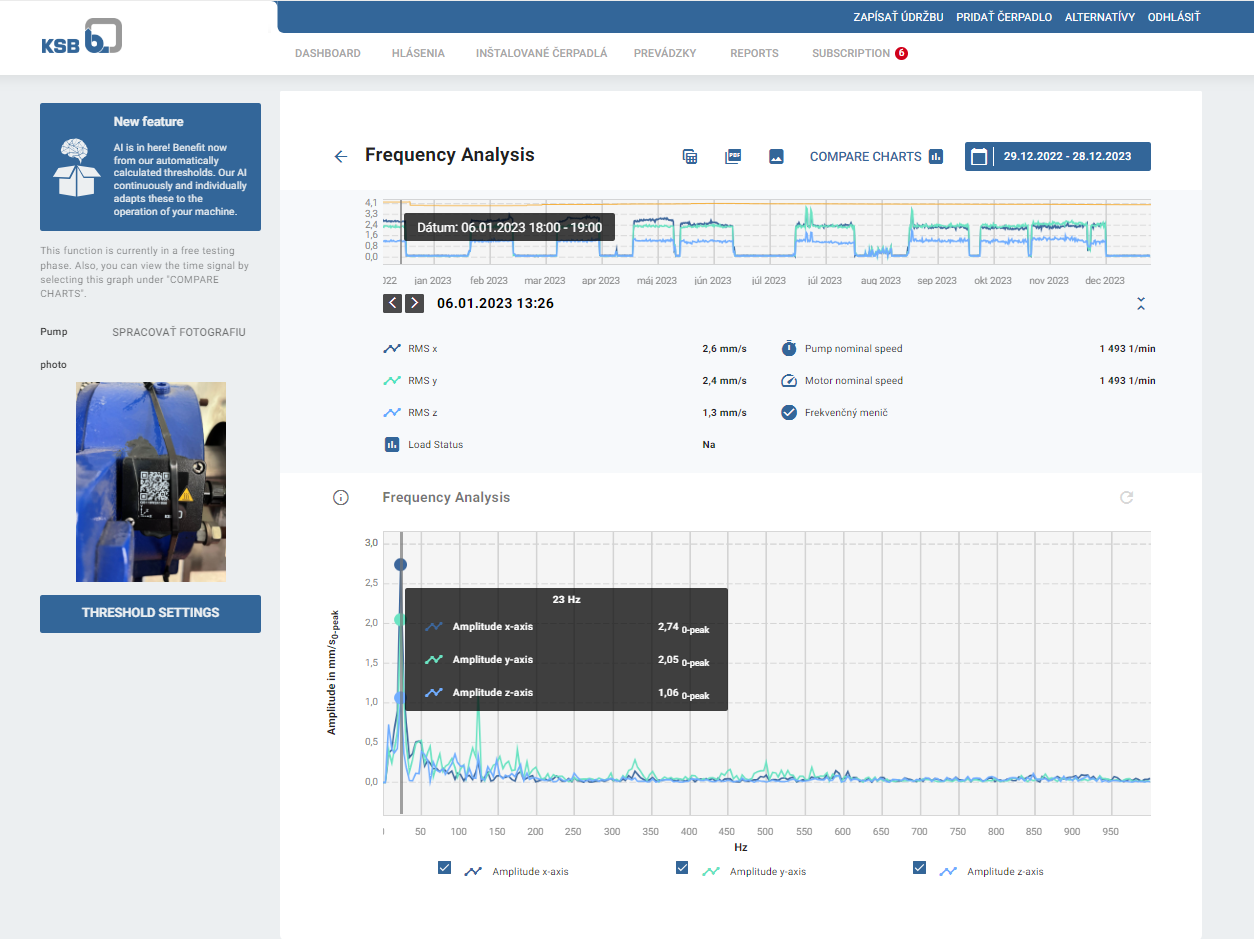
\includegraphics[width=\textwidth]{assets/design/ksb-guard-spectrum.png}
        \caption{Vibration spectral analysis dashboard}
    \end{subfigure}
     \caption{KSB Guard cloud monitoring for pumps}
     \label{fig:design:ksb-guard}
\end{figure}

\textbf{Complete schedule} for planned vibration data gathering on the designated machines and measurement procedure is described in Appendix~\ref{appendix:technical-docs}. In addition, we are able to export the entire historical record at hourly intervals. Logs from \textbf{KSB Guard} cloud monitoring tool contain vibration rms velocities and frequency spectra for two monitored KSB water pumps (Figure~\ref{fig:design:ksb-guard}).


\section{Data volume savings}
The apparent advantage of feature discovery is reducing the amount of data downstream. Data compression must occur on edge devices to enable the utilization of wireless low-power wide area networks (LPWAN). The protocol stack may differ, so goodput is compared without node configuration metadata and keepalive messages. 

The machinery monitoring system relies on determining several parameters:
\begin{itemize}
\itemsep0pt
\item \textbf{Number of source channels} ($S$): comprises the number of monitored machines, measurement locations for sensors, and active sensor axes.
\item \textbf{Sampling frequency} ($f_s$): is set based on the linear response of the accelerometer, the types of faults intended for detection, and how soon they should be noticed after they arise. The higher required sensitivity means a higher sampling rate derived according to the Nyquist theorem. At a minimum, it should be 15 kHz to 20 kHz.
\item \textbf{Interval between successive measurements} ($T$): specifies the minimal response time to sudden failure. The more critical the machine is, the interval should be shorter. The bigger the machine parts, the slower the defect evolves.
\item \textbf{Duration of valid recording} ($D$): is the captured snapshot of machine unaltered behavior associated with a timestamp. Duration should cover at least 3 windows for spectral estimation. The spectral resolution of 1 Hz amounts to 3 seconds of signal under such assumptions.
\item \textbf{Number of extracted features} ($F$): are ideally key trend indicators pointing to symptoms of common malfunctions. We aim for a total of 6 features.
\end{itemize}

Equation \ref{equ:compression-ratio-features} expresses the lossy compression ratio ($\mathcal{C}$) formula if trend indicators are stored instead of full recording. The number of raw channels ($S_{\mathrm{in}}$) can differ from those extracted in features ($S_{\mathrm{out}}$). Parameter $D = 0.5$ when we use frequency bins with 1 Hz resolution.

\myequations{Lossy compression ratio with features}
\begin{ceqn}\begin{align} \label{equ:compression-ratio-features}
\mathcal{C} = \frac{D \cdot f_s \cdot S_{\mathrm{in}}}{F \cdot S_{\mathrm{out}}}
\end{align}\end{ceqn}

\textbf{Compression ratio} for MaFaulDa dataset compared to all 21 extracted features in 3 dimensions is 2381:1. If 6 features are kept, the compression is 25000:1, which is a saving of the original data by 99.996\%.

As an example to approximate required network goodput and storage in practice, we consider continuous vibration \textbf{monitoring for municipal water pumping station}. The station has 3 pumps and 3 electric motors. 

A pump and motor pair have 4 bearings together for drive end and non-drive end positions. Each position has a sensor mounted in 3 directions that makes a total of \emph{36 source channels}. The sampling frequency at each position is set to \emph{20 kHz}. The recordings have \emph{duration of 5 seconds} and are triggered regularly every 1 hour (\emph{8760 times per year}).

In a year, the system gathers 31.54 Gs (gigasamples) which is 58.74 GiB with a 16-bit ADC resolution. Reasonably precise spectral estimation with 10 thousand bins needs 3.15 Gs per year. On the other hand, 6 features out of each channel keep only 1.89 Ms per year for a lossy compression ratio of 16667:1. Low data volumes potentially enable feature selection and models to be offloaded directly to edge devices. The entire machine's history can be kept in a small flash memory module.


\section{Data collection methodology}
% UML of experiment

% Measurement plan (calendar and folders) - dataset schema



